\documentclass[tikz,border=6pt]{standalone}
\usepackage{amsmath,amssymb}
\usepackage{tikz}
\usetikzlibrary{decorations.pathmorphing, decorations.markings, arrows.meta, calc}
\begin{document}
% scale: 整体缩放, 1.0 比较适中，想大一点改 1.2
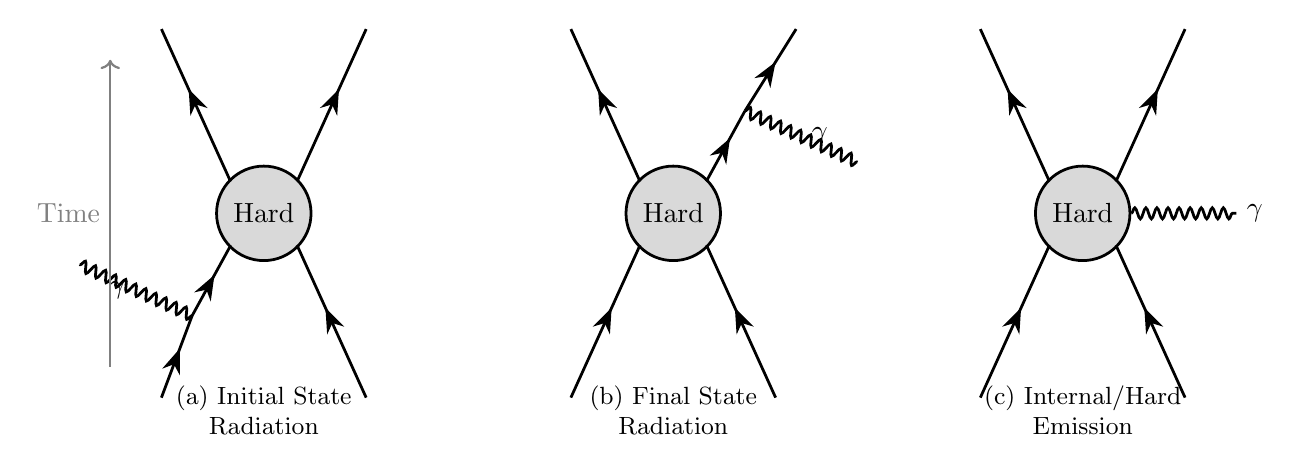
\begin{tikzpicture}[scale=1.3, line width=1pt,
    % --- 样式定义 ---
    photon/.style={decorate, decoration={snake, amplitude=2pt, segment length=4pt}},
    fermion/.style={postaction={decorate},
        decoration={markings,mark=at position 0.6 with {\arrow{Stealth[scale=1.2]}}}},
    % 硬过程Blob (灰色圆球)
    hard_blob/.style={circle, draw=black, fill=gray!30, minimum size=1.2cm, inner sep=0pt},
    % 图注文字样式
    caption/.style={text width=3cm, align=center, font=\small, yshift=-2.5cm}
]

    % =========================================
    % 【图 1】 ISR: 初态辐射 (入射腿发射)
    % 向左平移 4 个单位
    % =========================================
    \begin{scope}[shift={(-4, 0)}]
        \node[hard_blob] (b1) at (0,0) {Hard};
        
        % 1. 正常的腿 (右下入，两上出)
        \draw[fermion, shorten >= -1pt] (1, -1.8) -- (b1.315);
        \draw[fermion, shorten <= -1pt] (b1.135) -- (-1, 1.8);
        \draw[fermion, shorten <= -1pt] (b1.45)  -- (1, 1.8);

        % 2. 发射光子的腿 (左下入)
        \coordinate (in_start) at (-1, -1.8);
        \coordinate (emit_pos) at (-0.7, -1.0); % 发射点位置

        % 第一段：从无穷远 -> 发射点
        \draw[fermion] (in_start) -- (emit_pos);
        % 第二段：从发射点 -> Blob
        \draw[fermion, shorten >= -1pt] (emit_pos) -- (b1.225);
        
        % 3. 光子 (向左飞出)
        \draw[photon] (emit_pos) -- (-1.8, -0.5) node[midway, left] {$\gamma$};

        % 标签
        \node[caption] at (0, 0) {(a) Initial State\\ Radiation};
    \end{scope}

    % =========================================
    % 【图 2】 FSR: 末态辐射 (出射腿发射)
    % 居中 (不平移)
    % =========================================
    \begin{scope}[shift={(0, 0)}]
        \node[hard_blob] (b2) at (0,0) {Hard};

        % 1. 正常的腿 (两下入，左上出)
        \draw[fermion, shorten >= -1pt] (-1, -1.8) -- (b2.225);
        \draw[fermion, shorten >= -1pt] (1, -1.8)  -- (b2.315);
        \draw[fermion, shorten <= -1pt] (b2.135) -- (-1, 1.8);

        % 2. 发射光子的腿 (右上出)
        \coordinate (emit_pos_2) at (0.7, 1.0); % 发射点
        \coordinate (out_end)    at (1.2, 1.8);

        % 第一段：Blob -> 发射点
        \draw[fermion, shorten <= -1pt] (b2.45) -- (emit_pos_2);
        % 第二段：发射点 -> 无穷远
        \draw[fermion] (emit_pos_2) -- (out_end);

        % 3. 光子 (向右飞出)
        \draw[photon] (emit_pos_2) -- (1.8, 0.5) node[midway, right] {$\gamma$};

        % 标签
        \node[caption] at (0, 0) {(b) Final State\\ Radiation};
    \end{scope}

    % =========================================
    % 【图 3】 Internal: 硬区域直接发射
    % 向右平移 4 个单位
    % =========================================
    \begin{scope}[shift={(4, 0)}]
        \node[hard_blob] (b3) at (0,0) {Hard};

        % 1. 所有的腿都是直的
        \draw[fermion, shorten >= -1pt] (-1, -1.8) -- (b3.225);
        \draw[fermion, shorten >= -1pt] (1, -1.8)  -- (b3.315);
        \draw[fermion, shorten <= -1pt] (b3.135) -- (-1, 1.8);
        \draw[fermion, shorten <= -1pt] (b3.45)  -- (1, 1.8);

        % 2. 光子从 Blob 表面长出来
        % 从右侧 (角度0) 出来
        \draw[photon] (b3.0) -- (1.5, 0) node[right] {$\gamma$};

        % 标签
        \node[caption] at (0, 0) {(c) Internal/Hard\\ Emission};
    \end{scope}

    % --- 时间轴 (公用) ---
    \draw[->, thick, gray] (-5.5, -1.5) -- (-5.5, 1.5) node[midway, left] {Time};

\end{tikzpicture}
\end{document}
